\chapter{\IfLanguageName{dutch}{Stand van zaken}{State of the art}}%
\label{ch:stand-van-zaken}

% Tip: Begin elk hoofdstuk met een paragraaf inleiding die beschrijft hoe
% dit hoofdstuk past binnen het geheel van de bachelorproef. Geef in het
% bijzonder aan wat de link is met het vorige en volgende hoofdstuk.

% Pas na deze inleidende paragraaf komt de eerste sectiehoofding.


\section{Data Leakage Prevention (DLP)}%

Een DLP-systeem heeft als doel drie soorten gegevens binnen een organisatie te beschermen: data-at-rest, data-in-motion en data-in-use. 
Data-at-rest verwijst naar statische informatie die is opgeslagen in bedrijfssystemen, zoals documentbeheersystemen, e-mailservers, bestandsservers, netwerkschijven, 
persoonlijke computers en opslagruimtenetwerken (SANs). 
Data-in-motion verwijst naar bedrijfsdata dat wordt verwerkt binnen het uitgaande netwerkverkeer, zoals e-mails en online verkeer. 
Data-in-use bestaat uit informatie die medewerkers gebruiken op eindgebruikersapparaten, zoals een bestand kopiëren naar een USB-schijf. 
De definitie van vertrouwelijkheid binnen een organisatie vereist een grondigere analyse. 
Soorten informatie zoals PII, inclusief namen, identiteitskaart- en creditcardgegevens, worden doorgaans in elke organisatie als vertrouwelijk beschouwd.
Deze definitie krijgt echter ingewikkeldere aspecten bij bedrijfsgeheimen en interne communicatie, die vaak onregelmatig zijn. 
Vertrouwelijke informatie verwijst naar gegevens die binnen de organisatie zijn verzameld en niet algemeen toegankelijk zijn. 
Een DLP-systeem bevat de mogelijkheid om gevoelige gegevens te herkennen in een of meerdere van de genoemde datatypen.

\subsection{PCI en PII}

Persoonlijk identificeerbare informatie (PII), zoals namen, rijksregisternummers, e-mail\-adressen, telefoonnummers en dergelijke kunnen direct of indirect worden gebruikt voor de identificatie van een persoon. 
Met het oog op de AVG zijn er strikte regels met betrekking tot toestemming en transparantie bij de verwerking van PII. 
Payment Card Industry (PCI)-gegevens bevatten alle kaart- en betaalgegevens zoals debit-/creditcardnummers, Primary Account Numbers (PAN) en andere confidentiële authenticatiegegevens zoals CVV. 
Om te voldoen aan de PCI DSS-norm (Payment Card Industry Data Security Standard), 
moeten organisaties strenge maatregelen implementeren om deze kaartgegevens te beveiligen. 
Bedrijven die persoonlijk identificeerbare informatie (PII) en PCI-data verwerken lopen het risico op zware sancties als deze gegevens niet voldoende beschermd worden.

\subsection{Gegevensverlies detectie methoden}

Identificatiemiddelen worden gebruikt om gevoelige informatie, zoals PII en PCI, te detecteren. 
Dit gebeurt op basis van reguliere expressies (regex). 
Regex is een krachtig hulpmiddel dat DLP helpt specifieke gegevenstypen te herkennen door middel van uitdrukkingen, termen en patronen, 
zoals \texttt{BE\textbackslash d\{2\}\textbackslash s?\textbackslash d\{4\}\textbackslash s?\textbackslash d\{4\}\-\textbackslash s?\textbackslash d\{4\}} 
dat kan dienen voor Belgische IBAN-codes. Hoewel dit patroon effectief is voor standaard IBAN-formaten, kan het worden omzeild door een karakter toe te voegen in de invoer, 
wat de nood benadrukt van extra controles. 

De aangemaakte identificatie voor confidentiële gegevens moet voldoen aan de volgende richtlijnen:

\begin{itemize}
    \item Vooraf gedefinieerde en aanpasbare patronen voor datadetectie: Het is cruciaal om duizenden vooraf ingestelde regels voor het herkennen van gegevens beschikbaar te hebben en deze te kunnen aanpassen aan de behoeften van de organisatie.
    \item Ondersteuning voor verschillende soorten bestandstypen (Word, Excel, PDF, JPG, PNG, CSV, ZIP en RAR, enz.) en categorieën (afbeeldingen, databases, spreadsheets, enz.).
    \item Ondersteuning voor landspecifieke identificatienummers (IBAN's, postcodes, adressen, nationale identiteitskaarten, IP-adressen, pas\-poort- en telefoonnummers).
    \item Voldoen aan de wet- en regelgeving.
\end{itemize}

De bescherming van PII en PCI-gegevens vormt een kernaspect van DLP. \textcite{Wason2020CASB} legt de nadruk op het belang van de integratie van Cloud Access Security Brokers (CASB) in cloudomgevingen. 
CASB biedt organisaties de mogelijkheid om een uitgebreide zichtbaarheid te krijgen in het gebruik van cloudtoepassingen, inclusief goedgekeurde en ongeautoriseerde (shadow IT) diensten. 
Het houdt bij hoe de confidentiële data wordt opgeslagen en verplaatst/verwerkt, wat handig is voor het identificeren van deze data en het voorkomen van datalekken.

\subsection{\IfLanguageName{dutch}{Regelsets}{Rule sets}}
\label{subsec:regelsets-literatuurstudie}

De regelsets binnen Netskope zijn de focus van dit onderzoek. En bestaan uit een combinatie van verschillende identificatiemethoden, zoals beschreven in de documentatie van \textcite{Netskope2025DLP}. 
Deze identificatoren of ook entiteiten genoemd, zijn de bouwstenen van de DLP-regels en vormen samen een regelset. 
Meerdere regelsets kunnen worden gedefinieerd binnen een profiel \autocite{Netskope2025Profiles}.


% A DLP profile is a collection of predefined or custom DLP rules, classifiers, and custom fingerprint rules. If any of the rules or classifiers match the content, then the DLP profile flags the content as a policy violation. Using predefined profiles let you start evaluating loss of critical data in the cloud immediately. Creating new DLP profiles and rules enables you to refine custom methods of prevention. For insight about building custom DLP profiles and rules, see DLP Best Practices Runbook.

{\small
\begin{itemize}
    \item \textbf{Predefined data identifiers}: Dit zijn vooraf gedefinieerde identificatoren die zijn ontworpen door Netskope.
    \item \textbf{Custom data identifiers}: Dit zijn op maat gemaakte identificatoren die organisaties kunnen definiëren om specifieke soorten gevoelige gegevens te herkennen die relevant zijn voor hun bedrijfsvoering.
    \item \textbf{Keyword identifiers}: Dit zijn specifieke woorden of zinnen die worden gebruikt om gevoelige gegevens te identificeren. Dit kan bijvoorbeeld een lijst zijn van veelvoorkomende achternamen die in combinatie met een rijksregisternummer kunnen worden gebruikt.
    \item \textbf{Regular expressions (RegEx)}: Dit zijn patronen die worden gebruikt om specifieke gegevensformaten te identificeren. RegEx kan worden gebruikt om complexe gegevensstructuren te herkennen, zoals IBAN-nummers of e-mailadressen.
    \item \textbf{Exact match criteria}: Dit zijn specifieke voorwaarden die moeten worden vervuld om te bepalen of een gegevenstype als gevoelig wordt beschouwd, zoals 
\end{itemize}
}


\subsubsection{\IfLanguageName{dutch}{Vooraf gedefinieerde regelsets}{Predefined rules}}
\label{subsubsec:vooraf-gedefinieerde-regels-literatuurstudie}

Netskope biedt een uitgebreide set vooraf gedefinieerde regelsets binnen zijn DLP-functionaliteit. 
Hiermee kan gevoelige informatie, zoals PII en PCI, effectief worden gedetecteerd en beschermd.
Volgens \textcite{brouwer2021cloud} heeft Netskope een uitgebreide lijst van DLP-profielen ontwikkeld die helpen bij het identificeren van allerlei soorten PII,
verschillend van EU-identificatiegegevens tot Singaporese identificatiegegevens en medische rapporten. 
Deze regelsets zijn uitgebalanceerd en sluiten aan bij de regelgeving van de meeste westerse landen. 

Deze vooraf gedefinieerde regelsets zijn niet veranderbaar en kunnen niet verder worden gepersonaliseerd. 
Gebruikers kunnen echter wel hun eigen DLP-profielen definiëren voor specifieke use-cases, zoals in volgende sectie wordt besproken. 

Een voorbeeld van een vooraf gedefinieerde regelset is de regelset voor 'DLP-PII', die is ontworpen om gevoelige persoonlijke informatie te identificeren en te beschermen. 
Deze regelset omvat gegevens zoals naam, adres, geboortedatum, e-mailadres, MedicareID, paspoortinformatie en sociale zekerheidsnummers. Alleen zijn deze specifiek gericht voor de Verenigde Staten en Canada. 
Aangezien dit onderzoek zich richt op de bescherming van Belgische persoons\-- en betalingsgegevens, voldoet deze regelset niet aan de vereisten van de Belgische wetgeving.

Daarnaast biedt Netskope ook de 'EU General Data Protection Regulation (GDPR)' regelset aan, die specifiek is ontworpen om te voldoen aan al de vereisten van de AVG. 
Deze regelset richt zich op persoonsgegevens van een natuurlijk persoon binnen de Europese Unie. 
In Tabel \ref{tab:EU-AVG Netskope} zijn de gegevenscategorieën weergegeven die Netskope heeft gedefinieerd voor deze regelset \autocite{Netskope2023GDPR}. 
De entiteit/ dataset zelf is niet publiek beschikbaar, dus zal deze aan de hand van een steekproefevaluatie worden beoordeeld. 

\begin{table}[h]
    \centering
    \small
    \begin{tabular}{p{5cm}p{10cm}}
    \toprule
    \textbf{Categorie} & \textbf{Gegevens} \\
    \midrule
    Adres & PAN Vervaldatum, Naam, IP-adres, Telefoonnummer, E-mail, Region, Region-Date \\
    Rijbewijs & Geboortedatum, Naam, Adres, Geslacht, Rijbewijsnummer, Uitgiftedatum, Vervaldatum \\
    Identiteit & Biometrische gegevens, Geboortedatum, Naam, Geslacht, Etniciteit, Religie, Lengte, Gewicht, Haarkleur, Oogkleur, Gezondheidsgegevens, Handtekening, Nationaal Identificatienummer \\
    Naam & PAN, IP-adres, Telefoonnummer, E-mail, Politieke voorkeur, Criminele geschiedenis, Religie, Etniciteit, Geslacht, Lengte, Gewicht, Haarkleur, Oogkleur, Voorkeursnaam, Alias \\
    Paspoort & Naam, Adres, Geboortedatum, Biometrische gegevens, Paspoortnummer, Uitgifteland, Uitgiftedatum, Vervaldatum \\
    \bottomrule
    \end{tabular}
    \caption{Data categorieën van EU-AVG-ruleset \autocite{Netskope2023GDPR}}
    \label{tab:EU-AVG Netskope}
\end{table}

\subsubsection{\IfLanguageName{dutch}{Aangepaste regelsets}{Custom rules}}
\label{subsubsec:aangepaste-regels-literatuurstudie}

De focus van dit onderzoek ligt op de aangepaste regelsets, zoals besproken in Hoofdstuk \ref{ch:proofofconcept}. 
Elke regelset, oftewel profiel genoemd, bestaat uit DLP-regels, content classificaties of fingerprintregels \autocite{Netskope2025CreateProfiles}.
Elke regel bestaat uit een of meerdere entiteiten, die elk een specifiek type gegevens identificeren. 
Dit kan bijvoorbeeld een specifieke reeks cijfers zijn die overeenkomt met een rijksregisternummer of een reeks woorden die samen een bepaalde context vormen, zoals een naam in de buurt van een adres. 

\subsection{\IfLanguageName{dutch}{Entiteit}{Entity}}
\label{subsec:entiteit-literatuurstudie}

De entiteit is de basis van een DLP-regel. 
Deze entiteit houdt verschillende vormen van gegevens bij, zoals een reeks cijfers, woorden of zinnen. 
Dit onderzoek basseert zich op het gebruik van de entiteit 'Exact Match' en 'Regular Expression'. 
De configuratie gebruikt standaard de vooraf gedefinieerde entiteiten van Netskope. 
Als Netskope voor een specifieke behoefte geen vooraf gedefinieerde entiteit voorziet, dan zal een aangepaste entiteit worden aangemaakt.
Deze aangepaste entiteiten zullen vooral bestaan uit 'Exact Match', aangezien regex-regels, dankzij hun complexiteit, meer false positives kunnen genereren.

% \subsection{\IfLanguageName{dutch}{Fingerprint}{Fingerprint}}
% \label{subsec:fingerprint-literatuurstudie}

% MOCHT IK FINGERPRINTS GEBRUIKEN, DAN ZAL IK DIT VERDER AANVULLEN

\subsection{False Positives}
\label{sec:false-positives-literatuurstudie}

False positives ontstaan wanneer het DLP-syst\-eem onterecht normale gegevens als confidentieel identificeert. 
Dit kan leiden tot onnodige waarschuwingen en vertragingen in de bedrijfsprocessen. 
Om false positives te vermijden, kan in Netskope bij custom identifiers worden aangegeven dat een bepaald keyword in de buurt moet staan, zoals `RRN' of `Rijksregisternummer'. 
Hierdoor ziet Netskope het niet als een match of zal het een lagere vertrouwheidsscore geven. 

\subsection{Detectienauwkeurigheid}
\label{sec:detectienauwkeurigheid-literatuurstudie}

Detectienauwkeurigheid houdt in hoe goed het DLP-systeem in staat is om confidentiële gegevens te identificeren. 
Een hogere detectienauwkeurigheid wordt bereikt door het gebruik van goed afgestemde regelsets en geavanceerde herkenningsmethoden, zoals reguliere expressies (regex), keywords en contextuele analyse.
Netskope maakt gebruik van predefined datasets voor het verbeteren van de detectienauwkeurigheid. 
Deze datasets bevatten gestructureerde gegevens zoals PII en bieden ondersteuning voor verschillende soorten eisen, waaronder de AVG \autocite{Clementelli2023}. 
Netskope maakt ook gebruik van een vertrouwheidsscore om de betrouwbaarheid van de gedetecteerde data te bepalen. 
Deze score helpt bij het evalueren van de waarschijnlijkheid dat bepaalde gegevens confidentieel zijn, 
wat nodig is voor het verminderen van false positives en false negatives. 
Om deze nauwkeurigheid te verhogen, kunnen regelsets aangepast worden aan nieuwe typen confidentiële data of veranderende bedrijfsprocessen.
In deze proof-of-concept wordt de detectienauwkeurigheid beoordeeld door de verhouding tussen true positives, false positives, 
false negatives en true negatives, samengevat in een Confusion Matrix \autocite{Microsoftn.d.}.

\subsection{Systeemimpact}
\label{sec:systeemimpact-literatuurstudie}

% Het meten van de systeemimpact is een belangrijk aspect van DLP-implementaties. 
% Indicatoren hierbij zijn CPU-gebruik, geheugengebruik, netwerklatentie, throughput en systeemstabiliteit. 
% CPU- en geheugengebruik toont aan hoeveel resources het DLP-systeem op de infrastructuur verbruikt. 
% Netwerklatentie en throughput meten de invloed op de netwerkprestaties, 
% terwijl systeemstabiliteit aangeeft of het DLP-systeem consistent functioneert zonder storingen. 
% Voor het verzamelen en analyseren van deze gegevens kunnen tools zoals \textit{Performance Monitor}, 
% \textit{Nagios}, \textit{Zabbix} worden gebruikt. 

% \autocite{Netskope2025Utilization}

De implementatie van een DLP-oplossing kan een merkbare impact hebben op de prestaties van een IT-systeem,
wat invloed heeft op de workflow en gebruikerservaring van de eindgebruikers. 
Netskope heeft een cloudgebaseerde architectuur die het mogelijk maakt om DLP-regels in real-time toe te passen op zowel in- als uitgaand netwerkverkeer.
Deze deep content inspection toepassing houdt in dat Netskope continu gegevens inspecteert en analyseert. 
Afhankelijk van de configuratie en de hoeveelheid netwerkverkeer kan dit leiden tot een verhoogd CPU- en geheugengebruik bij de eindgebruikers,
vooral wanneer er meerdere complexe DLP-regels actief zijn.
Volgens de documentatie van \textcite{Netskope2025Utilization} functioneert de DLP-oplossing stabiel onder productielast, 
zolang het correct is afgestemd op de infrastructuur en het netwerkverkeer.
Tenslotte spelen netwerklatentie, throughput ook een belangrijke rol in de gebruikerservaring.
\textcite{Netskope2021SLA} heeft een Service Level Agreement (SLA) opgesteld die garandeert dat de latentie voor niet-gedecodeerd verkeer minder dan 10 milliseconden bedraagt.
Voor gedecodeerd verkeer, zoals SSL/TLS-verkeer dat wordt ontsleuteld voor inspectie, is de latentie gegarandeerd onder de 50 milliseconden.
Aangezien deze SLA-waarden bijzonder laag liggen, voert dit onderzoek hierover geen diepgaande technische analyse uit.
In plaats daarvan evalueert dit onderzoek de impact vanuit het perspectief van de eindgebruikers en verwerkt deze in de gebruikersevaluatie.

% \begin{itemize} 
%     \item Gemiddelde netwerklatentie (ms) tijdens het uploaden/downloaden van documenten bij actieve DLP-inspectie. 
%     \item Gemiddeld CPU-gebruik (\%) op endpoints of virtuele machines waar Netskope agents draaien. 
%     \item Aantal policy violations per minuut, als indicatie van het verwerkingsvolume en de effectiviteit van de regelsets. 
% \end{itemize}

\section{Netskope}%
\label{sec:netskope-literatuurstudie}

Netskope heeft zich ontwikkeld tot een vooraanstaande speler in cloudbeveiliging door zijn geavanceerde Secure Service Edge (SSE)-platform. 
Het levert geïntegreerde CASB- en DLP-mogelijk\-heden. 
Volgens \textcite{Riley2018} onderscheidt Netskope zich met functies zoals flexibele regelconfiguraties en realtime-detectie van gevoelige data. 
\textcite{VanDerWalt2022} identificeren belangrijke aspecten binnen Secure Access Service Edge (SASE) frameworks die nog onvoldoende onderzoek bevatten,
onder meer netwerk- en beveiligingsdiensten in een cloudgebaseerde omgeving. 
Deze aspecten zijn onder andere de integratie van verschillende beveiligingscomponenten zoals Secure Web Gateways (SWG), CASB en Zero Trust Network Access (ZTNA). 
Hierbij dienen deze onderdelen samen te werken om een integrale beveiligingsstrategie te creëren. 
Om deze integratie van beveiligingscomponenten en Zero Trust-principes verder te versterken, 
is Netskope lid van de \textcite{SpectraAlliance2025}, een samenwerking tussen vier cybersecuritybedrijven: CrowdStrike, Okta, Proofpoint en Netskope.
Deze alliantie is gericht op het bieden van een sterke Zero Trust-architectuur door verschillende beveiligingsdomeinen samen te laten werken. 
Netskope levert hierbij expertise op het gebied van cloud- en webbeveiliging, met een sterke focus op DLP\- en CASB\--functionaliteiten.
Bovendien is er een toenemende vraag naar het ontwikkelen van API\--integraties voor Security Information and Event Management (SIEM)\--systemen, 
zodat gegevens uit verschillende bronnen effectief kunnen worden verzameld en geanalyseerd.

Bij het evalueren van DLP-oplossingen binnen een SASE-architectuur is Netskope gekozen vanwege de unieke combinatie van functionaliteiten en prestaties die het biedt, 
evenals de verhouding ten opzichte van andere oplossingen. In 2018 werd Netskope door \textcite{Hille2018} beschreven als een van de innovators voor Cloud Security Management Platforms, 
zoals te zien in Figuur \ref{fig:netskope}.  
Toen waren ze volgens \textcite{Hille2018} nog relatief onder de radar, maar met een zeer aantrekkelijk productaanbod. 
Dit aanbod is sindsdien verder uitgebreid en omvat nu een breed assortiment aan functies die zijn ontworpen om cloudarchitecturen te beschermen. 

In de meest recente Magic Quadrant voor Security Service Edge (SSE) positioneert Gartner Netskope opnieuw als Leader, zoals te zien in Figuur \ref{fig:netskope2024}.

\begin{figure}[h]
    \centering
    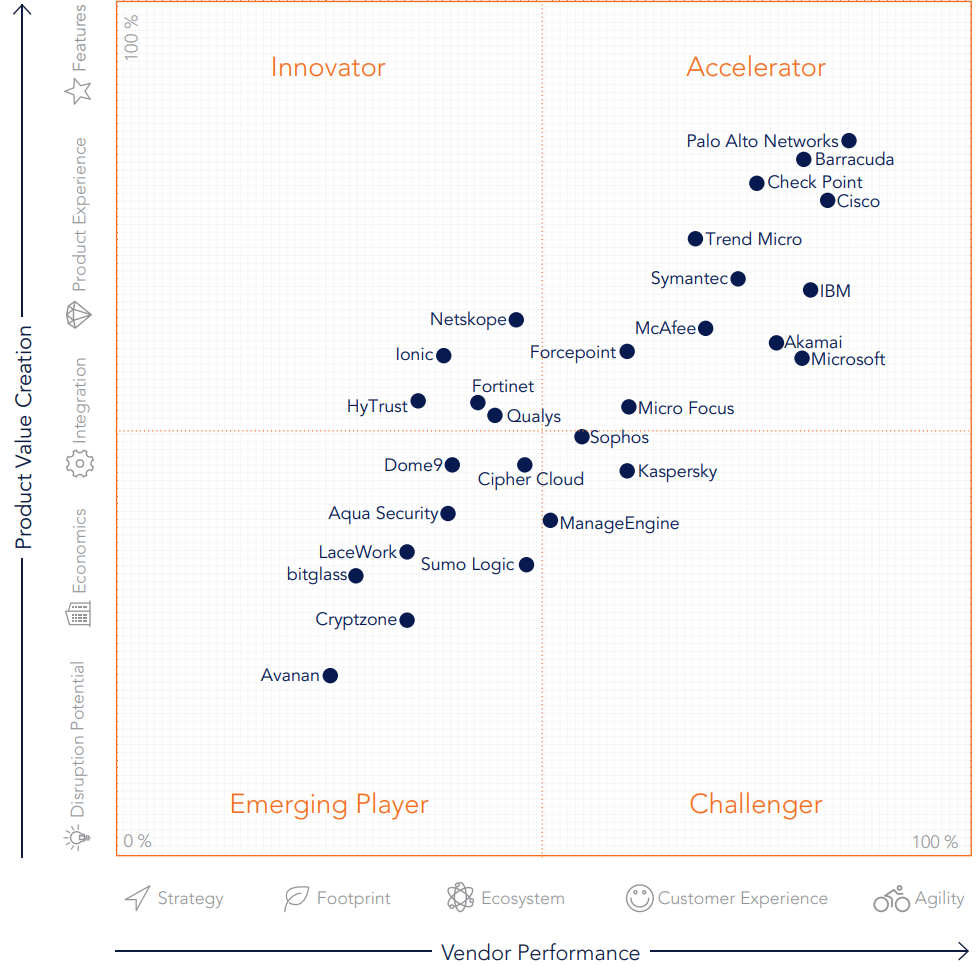
\includegraphics[width=0.8\textwidth]{img/netskopeinnovator.png}
    \caption{Quelle: Crisp Research AG, 2018 - Cloud Security Management Platforms \autocite{Hille2018}}
    \label{fig:netskope}
\end{figure}

\begin{figure}[h]
    \centering
    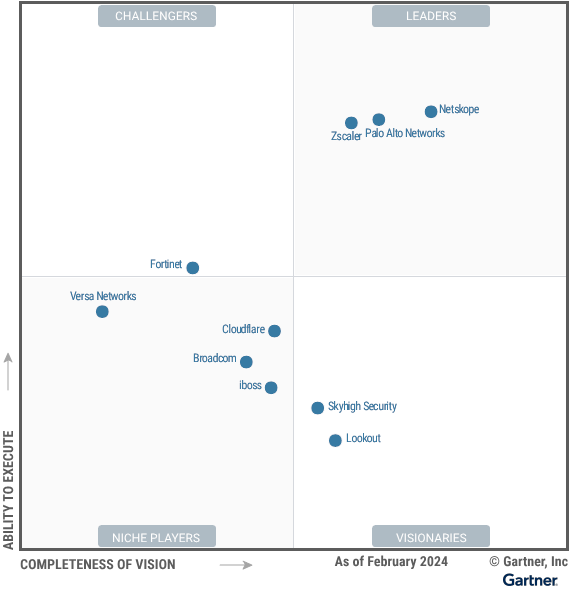
\includegraphics[width=0.8\textwidth]{img/netskope2024.png}
    \caption{Gartner Magic Quadrant voor Security Service Edge (SSE) \autocite{Gartner2024}}
    \label{fig:netskope2024}
\end{figure}


% Netskope onderscheidt zich als een volledig geïntegreerd platform binnen het SASE-framework, met een Secure Service Edge (SSE)-oplossing die DLP, CASB, SWG en ZTNA naadloos combineert. 
% Deze aanpak is waardevol in gedistribueerde werkomgevingen en bij toenemende cloudadoptie \autocite{brouwer2021cloud}. 
% Netskope biedt meer voordelen dan alternatieven zoals Symantec, Digital Guardian, Forcepoint, Microsoft en McAfee. 
% Symantec en Digital Guardian richten zich bijvoorbeeld sterk op endpointbeveiliging, maar missen de cloudfunctionaliteiten die nodig zijn in moderne hybride werkomgevingen. 
% Forcepoint staat bekend om krachtige gedragsanalyses, maar is minder effectief in het ondersteunen van complexe en dynamische cloudomgevingen. 
% Microsoft biedt uitstekende integratie met Office 365, maar hierdoor mist het ook Netskope's cloud-agnostische aanpak, die een breder scala aan cloudapplicaties ondersteunt \autocite{NetskopeTAP2024}. 
% Tenslotte biedt McAfee een breed scala aan beveiligingsoplossingen, maar voor Evolane is Netskope een gebruiksvriendelijker platform met meer flexibiliteit bij het opstellen en aanpassen van regelsets.




% O = onvoldoende
% V = voldoende
% G = goed
% U = uitstekend

% \begin{table}[h]
%     \centering
%     \small
%     \begin{tabular}{p{3cm} p{1.5cm} p{1.5cm} p{1.5cm} p{1.5cm} p{1.5cm} p{1.5cm}}
%         \toprule
%         & \textbf{Cloud-native} & \textbf{SASE/SSE} & \textbf{Flexibele regels} & \textbf{Endpoint focus} & \textbf{SIEM-integratie} & \textbf{Gebruiks\-vriendelijk} \\
%         \midrule
%         Netskope            & U & U & U & U & G & U \\
%         Symantec            & X & X & X & X & G & X \\
%         Microsoft           & X &   &   &   & Vthestral &   \\
%         Forcepoint          & X &   & X & X & G & X \\
%         Digital Guardian    &   &   &   & X &   &   \\
%         McAfee              & X &   & X & X &   &   \\
%         \bottomrule
%     \end{tabular}
%     \caption{Vergelijking van DLP-oplossingen per factor}
%     \label{tab:netskope}
% \end{table}




\section{Juridisch kader voor gegevensbescherming in België}%

De bescherming van persoonlijke en bedrijfsinformatie is een essentieel aspect van de hedendaagse digitale samenleving. 
Op zowel nationaal als Europees niveau zijn er wettelijke richtlijnen opgesteld om organisaties te ondersteunen bij het garanderen van de vertrouwelijkheid, 
integriteit en toegankelijkheid van gegevens.

\subsection{Algemene Verordening Gegevens\-besch\-erming (AVG)}%

Dit onderzoek zal in overeenstemming zijn met de Algemene Verordening Gegevensbescherming (AVG of GDPR) 2016/679 van 27 april 2016 \autocite{eu_avg2016} en de Belgische wet van 30 juli 2018 \autocite{BelgischeOverheid2018}.
Volgens de \textcite{eu_avg2016}, overweging (78), moeten passende, technische en organisatorische maatregelen worden genomen om de rechten van natuurlijke personen te beschermen. 
Deze overweging zorgt ervoor dat persoonsgegevens op een veilige en verantwoorde manier worden verwerkt. 
Zo'n beveiliging kan gebeuren door middel van standaardinstellingen die erop zijn gericht om risico's in elke fase van de verwerking van gegevens te minimaliseren.
Op 25 juli 2024 publiceerde de Europese Unie haar tweede verslag over de toepassing van de AVG \autocite{eu_avg2024}. 
Dit rapport legt de nadruk op het feit dat de AVG, ondanks verschillende uitdagingen, een goede basis is voor het veilig en transparant behandelen van persoonsgegevens. 


\subsection{Payment Card Industry Data Security Standard (PCI DSS)}%

De Payment Card Industry Data Security Stand\-ard (PCI DSS) bestaat uit een reeks richtlijnen en regels die ontworpen zijn voor organisaties die betalingsinformatie en kaartinformatie verwerken, 
zoals debit-/ creditcardnummers, Primary Account Numbers (PAN) en Sensitive Authentication Data (SAD), zoals Card Verification Value (CVV) en magnetische stripgegevens, van alle grote kaartsche\-ma's. 
Deze standaard is ontwikkeld om de veiligheid van kaartinformatie te garanderen en vereist dat organisaties maatregelen nemen om de gegevens van kaarthouders te beschermen \autocite{Elluri2018}. 
PCI DSS vereist de implementatie van toegangscontroles, zoals DCS-02 (toegangscontrole tot systemen en gegevens), DCS-07 (beheer van gebruikersidentiteiten en -toegang), 
en DCS-08 (toegangscontrole tot netwerken en systemen), om de veiligheid van kaartinformatie en de bescherming van kaarthoudergegevens te waarborgen \autocite{Elluri2018}.

\subsection{ISO 27001: Informatiebeveiliging}%

Bovendien moet de DLP-oplossing rekening houden met de vereisten van ISO 27001, de internationale norm voor het beheer van informatiebeveiliging. 
In dit verband bespreken \textcite{Alsanabani2020} de noodzaak van DLP-oploss\-ingen die zowel detectie- als preventieve methoden samenbrengen. 
De preventieve aanpak probeert datalekken te vermijden door onder andere het gehele confidentiële bestand te versleutelen, toegangscontrole aan te passen en het labelen van de inhoud.

\subsection{Nationale en Europese richtlijnen}%

Buiten de Belgische wetgeving zijn er ook tal van Europese richtlijnen en nationale standaarden die een belangrijke rol hebben in de bescherming van bedrijfsdata. 
Hierbij kan gedacht worden aan de Algemene Verordening Gegevensbescherming (AVG), de EU Cybersecurity Act en belangrijke Europese richtlijnen, waaronder de NIS2-richtlijn. 
Deze richtlijnen worden verder uitgebreid met specifieke normen, zoals de PCI DSS voor betalingsgegevens en internationale normen, zoals ISO 27001 voor de beveiliging van informatie. 
De NIS2-richtlijn (Richtlijn (EU) 2022/2555), die op 16 januari 2023 is aangenomen door de \textcite{nis2directive}, 
heeft als doel de cyberbeveiliging binnen de EU te versterken door een hoog niveau van beveiliging te waarborgen voor netwerken en informatiesystemen. 
Artikel 21 van de NIS2-richtlijn richt zich op de beveiliging van netwerken en informatiesystemen en legt de verplichting op aan lidstaten om 
ervoor te zorgen dat aanbieders van essentiële en belangrijke diensten passende technische en organisatorische maatregelen nemen. 
Maatregelen die over het DLP-systeem kunnen gaan, zijn onder andere: 

\begin{itemize}
    \item Risicoanalyse (lid 2, punten a en e): Organisaties moeten een risicobeheerproces implementeren dat hen in staat stelt om risico's voor de beveiliging van netwerken en informatiesystemen te identificeren, te evalueren en te beheersen.
    \item Encryptie en toegangscontroles (lid 2, punten h en i): Het gebruik van encryptie, toegangscontroles en regelmatige beveiligingstests en audits.
    \item Incidentenbehandeling (lid 2, punt b): Organisaties moeten procedures en mechanismen hebben voor het detecteren, melden en reageren op beveiligingsincidenten.
    \item Bewustwording en training (lid 2, punt g): Opleidingen om medewerkers te informeren over goede cyberhygiëne en risicomanagement \autocite{nis2directive}. Het DLP-systeem van Netskope staat in voor het trainen van de eindgebruiker, mocht deze iets foutief doen.
\end{itemize}

De studie van \textcite{Nayak2020} geeft een uitgebreid overzicht van systemen voor het detecteren en voorkomen van datalekken, 
inclusief de indeling van systemen op basis van de status van de gegevens (data-at-rest, data-in-motion, dat\-a-in-use) en de detectietechnieken. 
Dit overzicht zal gebruikt worden voor het ontwikkelen van regex-gebaseerde regels in DLP-oploss\-ingen. 
De studie legt de nadruk op het feit dat datalekken zowel onvoorzien als opzettelijk kunnen optreden en geeft uitdagingen aan, 
zoals het identificeren van gevoelige informatie, het balanceren van de detectienauwkeurigheid en de integratie van geavanceerde methodologieën.

% \subsection{Gegevensoverdracht en internationale implicaties}%

\subsection{Andere relevante wetgeving}%

Tabel \ref{tab:wetgeving_dlp} bevat de belangrijkste wettelijke richtlijnen en uitspraken die relevant zijn voor het ontwerp en de implementatie van een Data Leakage Prevention-oplossing voor Belgische bedrijven.

% \begin{figure}
%     \centering
%     % \includegraphics[width=.2\textwidth]
%     \includegraphics[scale=0.50]
%     {img/overzicht.png}
%     \caption{\label{fig:overzicht}Overzicht van de belangrijkste wettelijke richtlijnen en uitspraken voor DLP-oplossingen in België.}
%   \end{figure}

  
  \begin{table}[h]
    \centering
    \small
    \begin{tabular}{p{4cm} p{5cm} p{6cm}}
        \toprule
        \textbf{Wetgeving} & \textbf{Doel} & \textbf{Relevantie voor DLP} \\
        \midrule
        AVG & Bescherming persoonsgegevens & Dataclassificatie en toegangscontrole \\
        PCI DSS & Beveiliging van betalingsgegevens & Encryptie en toegangsbeheer \\
        ISO 27001 & Informatiebeveiliging & Risicoanalyse en ISMS-implementatie \\
        CCB-framework & Strategie voor cybersecurity België & Aanbevelingen voor risicobeheer \\
        NIS2 & Beveiliging netwerken en diensten & Incidentrapportage en risicoanalyse \\
        EU Cybersecurity Act & Certificering van beveiligingstechnologie & DLP-oplossingen certificeren \\
        Schrems II & Gegevensoverdracht naar niet-EU-landen & Beperking van cloud-gebaseerde opslag \\
        \bottomrule
    \end{tabular}
    \caption{Overzicht van wetgeving en relevantie voor DLP}
    \label{tab:wetgeving_dlp}
\end{table}


  

\section{Ethische overwegingen}%

Een essentieel aspect van de implementatie van DLP is het vinden van de juiste balans tussen gegevensbeveiliging en gebruikersprivacy. 
Het gebruik van DLP-systemen kan leiden tot het monitoren van gebruikersgedrag, wat kan worden gezien als een inbreuk op de privacy van medewerkers. 
Om het vertrouwen bij medewerkers en klanten te behouden, is het belangrijk om transparant te zijn over het gebruik van DLP-systemen en de redenen daarvoor. 
Hierdoor weet elke gebruiker welke gegevens worden verzameld en hoe deze worden gebruikt \autocite{Zaini2024}. 
Deze regelsets moeten niet alleen voldoen aan de wettelijke vereisten, maar ook aan de ethische normen en waarden van de organisatie. 
Om monitoring van data en gebruikersgedrag te minimaliseren, 
zal de implementatie van de DLP-oplossing specifiek gericht zijn op het beschermen van gevoelige gegevens en het voorkomen van datalekken. 


% % Dit hoofdstuk bevat je literatuurstudie. De inhoud gaat verder op de inleiding, maar zal het onderwerp van de bachelorproef *diepgaand* uitspitten. De bedoeling is dat de lezer na lezing van dit hoofdstuk helemaal op de hoogte is van de huidige stand van zaken (state-of-the-art) in het onderzoeksdomein. Iemand die niet vertrouwd is met het onderwerp, weet nu voldoende om de rest van het verhaal te kunnen volgen, zonder dat die er nog andere informatie moet over opzoeken \autocite{Pollefliet2011}.

% % Je verwijst bij elke bewering die je doet, vakterm die je introduceert, enz.\ naar je bronnen. In \LaTeX{} kan dat met het commando \texttt{$\backslash${textcite\{\}}} of \texttt{$\backslash${autocite\{\}}}. Als argument van het commando geef je de ``sleutel'' van een ``record'' in een bibliografische databank in het Bib\LaTeX{}-formaat (een tekstbestand). Als je expliciet naar de auteur verwijst in de zin (narratieve referentie), gebruik je \texttt{$\backslash${}textcite\{\}}. Soms is de auteursnaam niet expliciet een onderdeel van de zin, dan gebruik je \texttt{$\backslash${}autocite\{\}} (referentie tussen haakjes). Dit gebruik je bijv. bij een citaat, of om in het bijschrift van een overgenomen afbeelding, broncode, tabel, enz. te verwijzen naar de bron. In de volgende paragraaf een voorbeeld van elk.

% % \textcite{Knuth1998} schreef een van de standaardwerken over sorteer- en zoekalgoritmen. Experten zijn het erover eens dat cloud computing een interessante opportuniteit vormen, zowel voor gebruikers als voor dienstverleners op vlak van informatietechnologie~\autocite{Creeger2009}.

% % Let er ook op: het \texttt{cite}-commando voor de punt, dus binnen de zin. Je verwijst meteen naar een bron in de eerste zin die erop gebaseerd is, dus niet pas op het einde van een paragraaf.

% % \begin{figure}
% %   \centering
% %   \includegraphics[width=0.8\textwidth]{grail.jpg}
% %   \caption[Voorbeeld figuur.]{\label{fig:grail}Voorbeeld van invoegen van een figuur. Zorg altijd voor een uitgebreid bijschrift dat de figuur volledig beschrijft zonder in de tekst te moeten gaan zoeken. Vergeet ook je bronvermelding niet!}
% % \end{figure}

% % \begin{listing}
% %   \begin{minted}{python}
% %     import pandas as pd
% %     import seaborn as sns

% %     penguins = sns.load_dataset('penguins')
% %     sns.relplot(data=penguins, x="flipper_length_mm", y="bill_length_mm", hue="species")
% %   \end{minted}
% %   \caption[Voorbeeld codefragment]{Voorbeeld van het invoegen van een codefragment.}
% % \end{listing}

% % \lipsum[7-20]

% % \begin{table}
% %   \centering
% %   \begin{tabular}{lcr}
% %     \toprule
% %     \textbf{Kolom 1} & \textbf{Kolom 2} & \textbf{Kolom 3} \\
% %     $\alpha$         & $\beta$          & $\gamma$         \\
% %     \midrule
% %     A                & 10.230           & a                \\
% %     B                & 45.678           & b                \\
% %     C                & 99.987           & c                \\
% %     \bottomrule
% %   \end{tabular}
% %   \caption[Voorbeeld tabel]{\label{tab:example}Voorbeeld van een tabel.}
% % \end{table}

